\renewcommand{\abstractname}{Resumen}

\section*{Corpus}
\subsection*{CorpusLogo}
\begin{frame}
    \centering %Figura centrada.
    
\includegraphics[width=150px]{Assets/corpus_logo.png}
\end{frame}

\subsection*{Constructor}
\begin{frame}
    \begin{abstract}
        El constructor de esta clase se encargará, de forma no irónica, construir el Contenedor de documentos, palabras y datos de estos mismos
        \begin{center}
            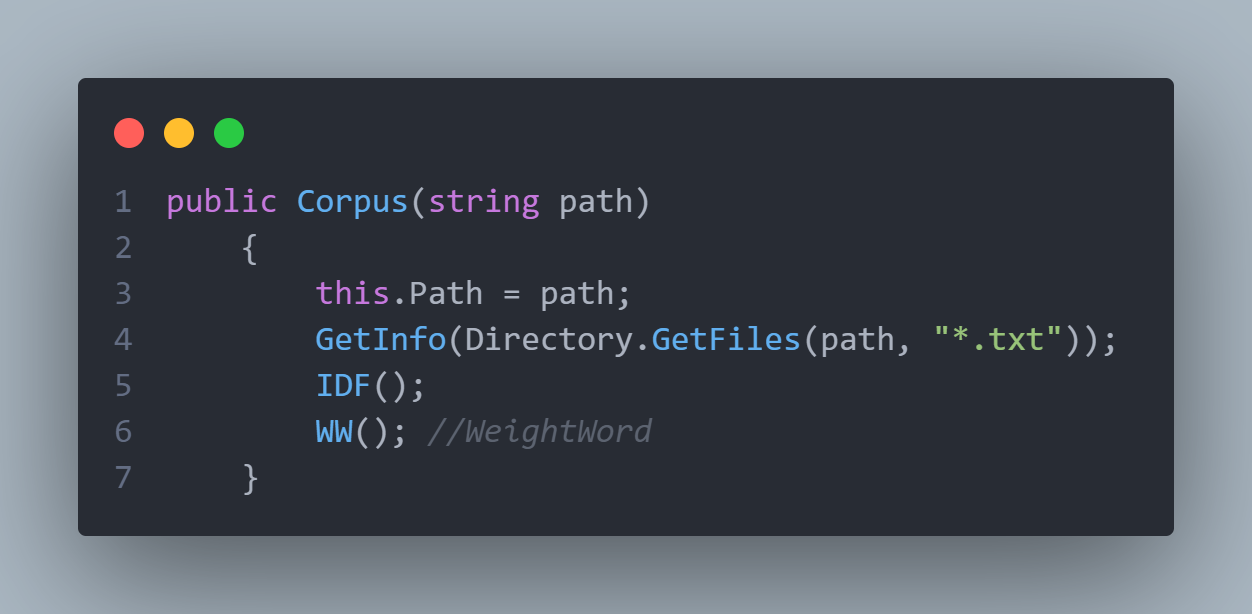
\includegraphics[width=250px]{Assets/corpus_constructor.png} 
        \end{center}
        *Nota: Cada función presente en esta presentación estan explicadas por orden en el Informe!
    \end{abstract}
\end{frame}

\begin{frame}
    Aquí cabe destacar la función principal que va recolectando y procesando cada documento destinado.
    \begin{figure}
        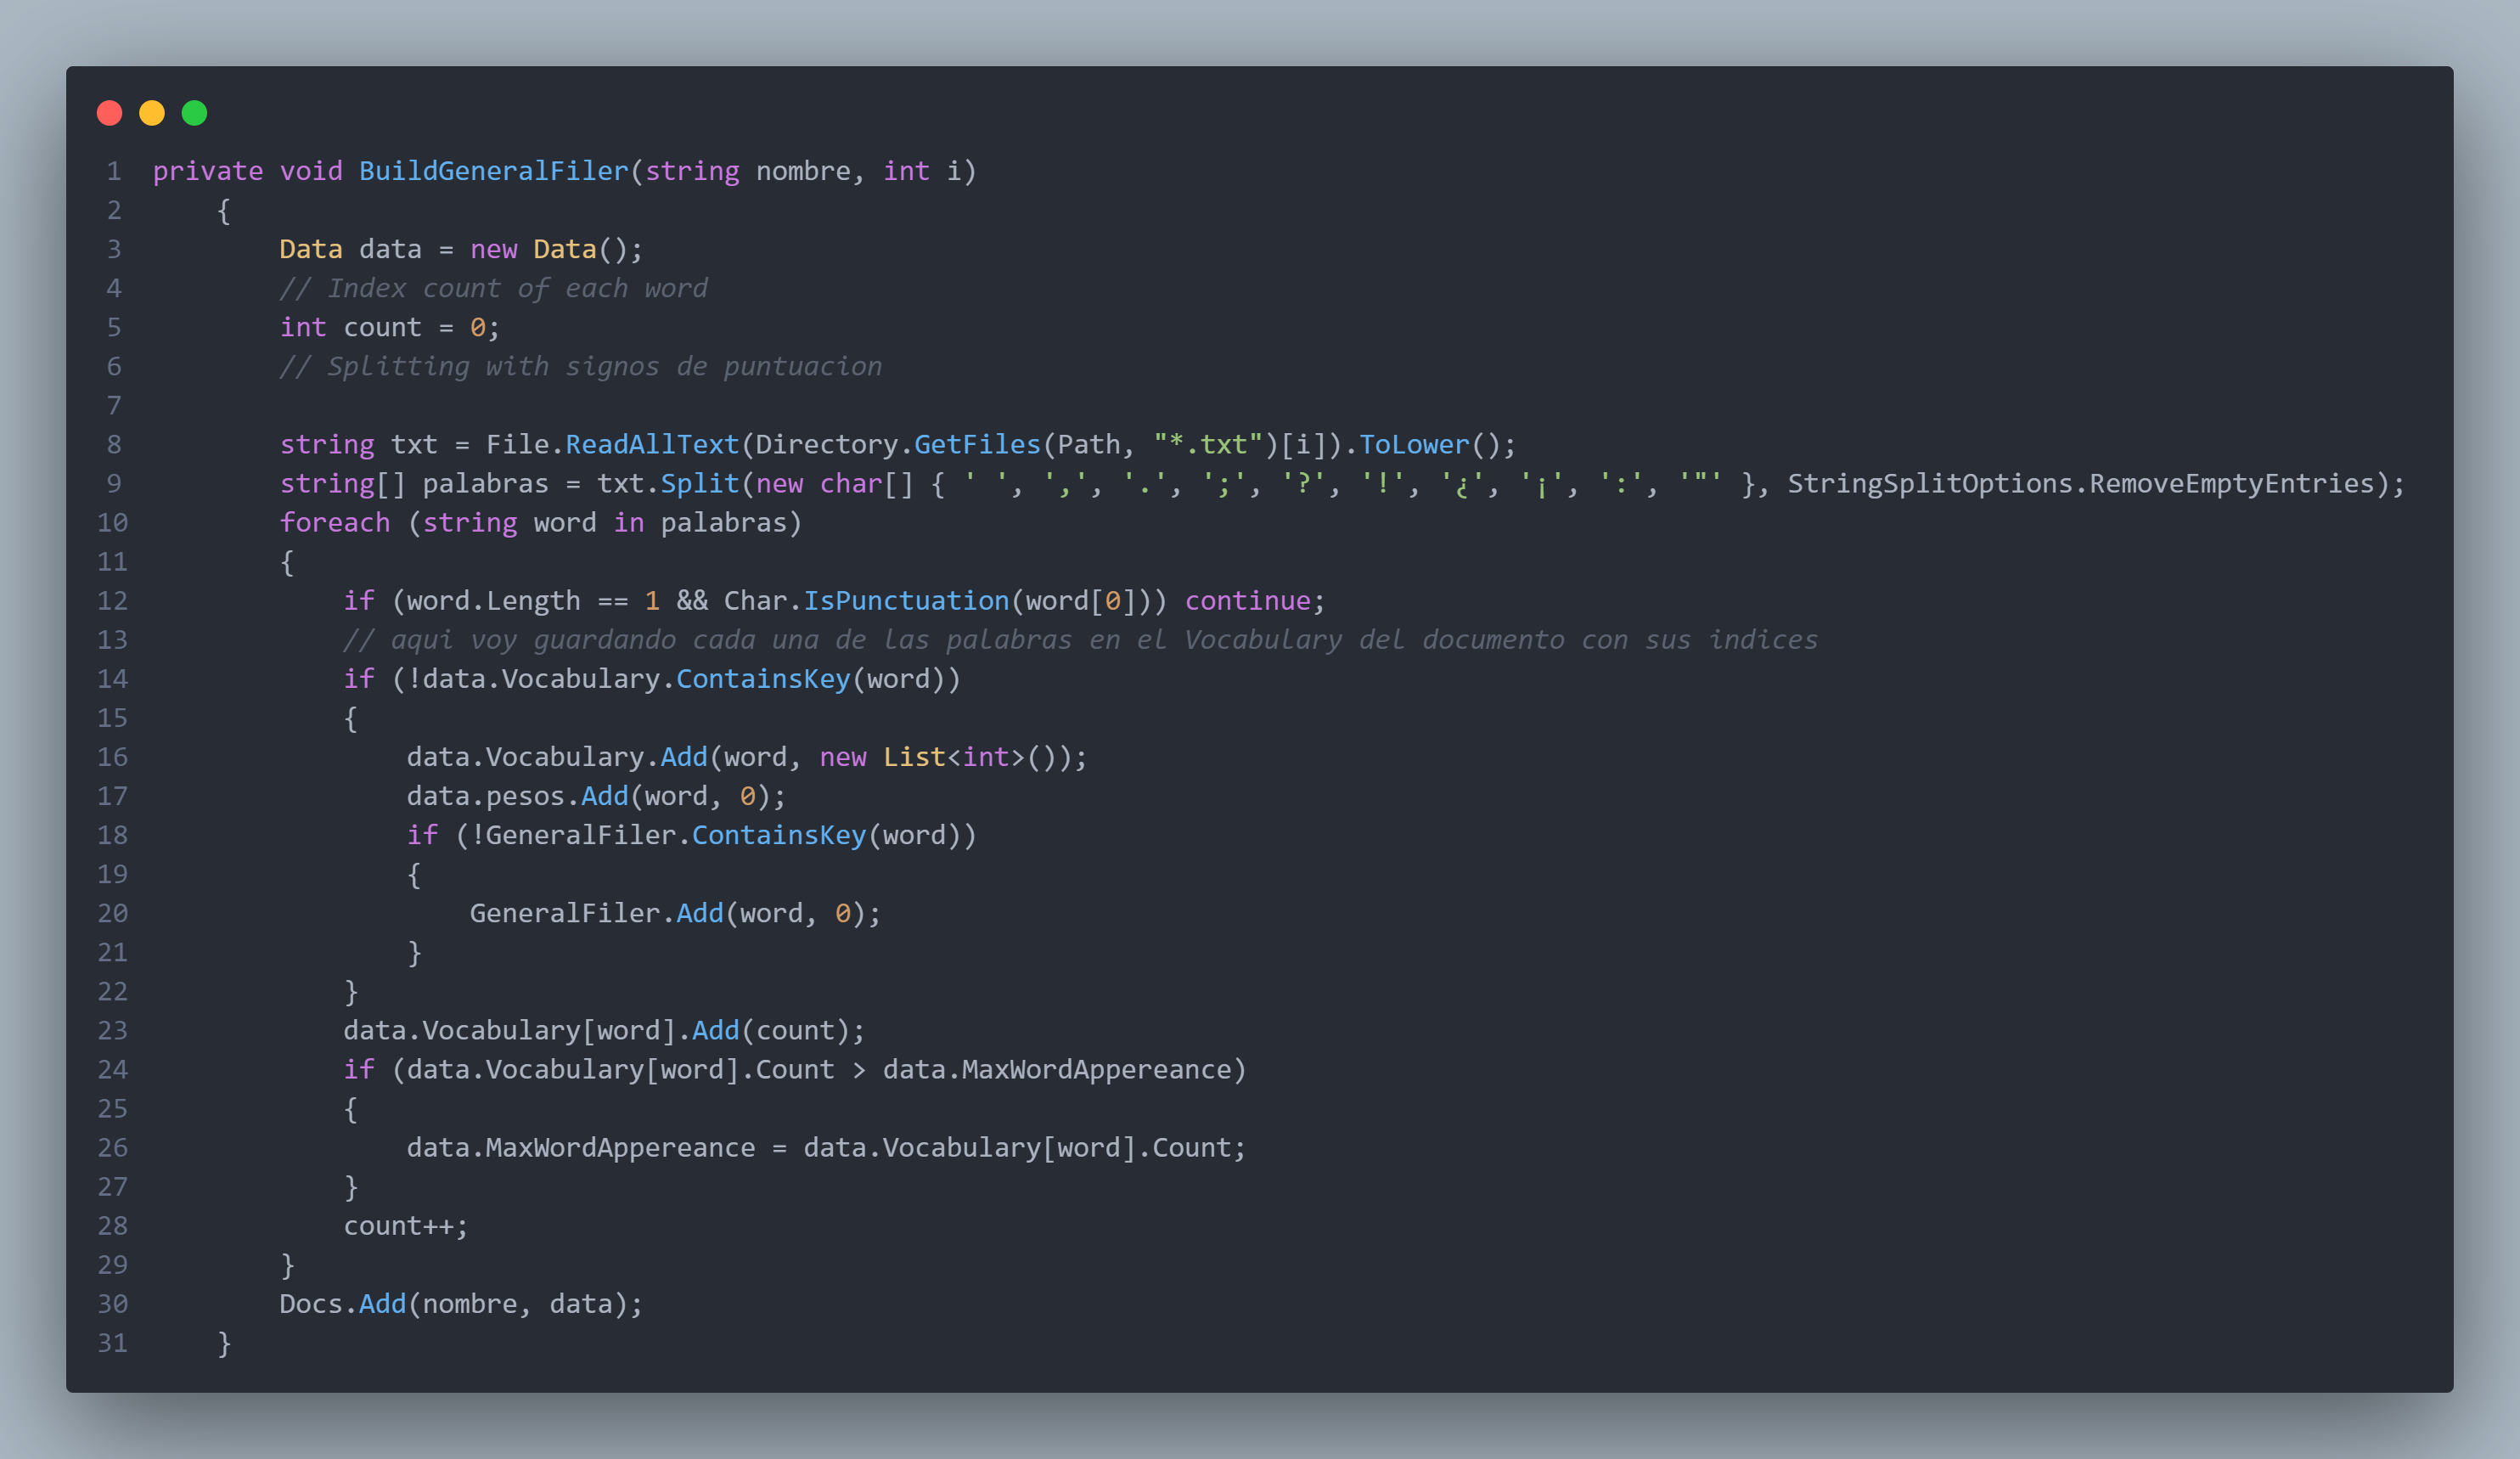
\includegraphics[width=280px]{Assets/general_filer.png}
    \end{figure}
\end{frame}


\begin{frame}
    En la anterior figura se vió como al inicio se instanciaba un objeto data, de tipo Data\dots
    \begin{figure}
        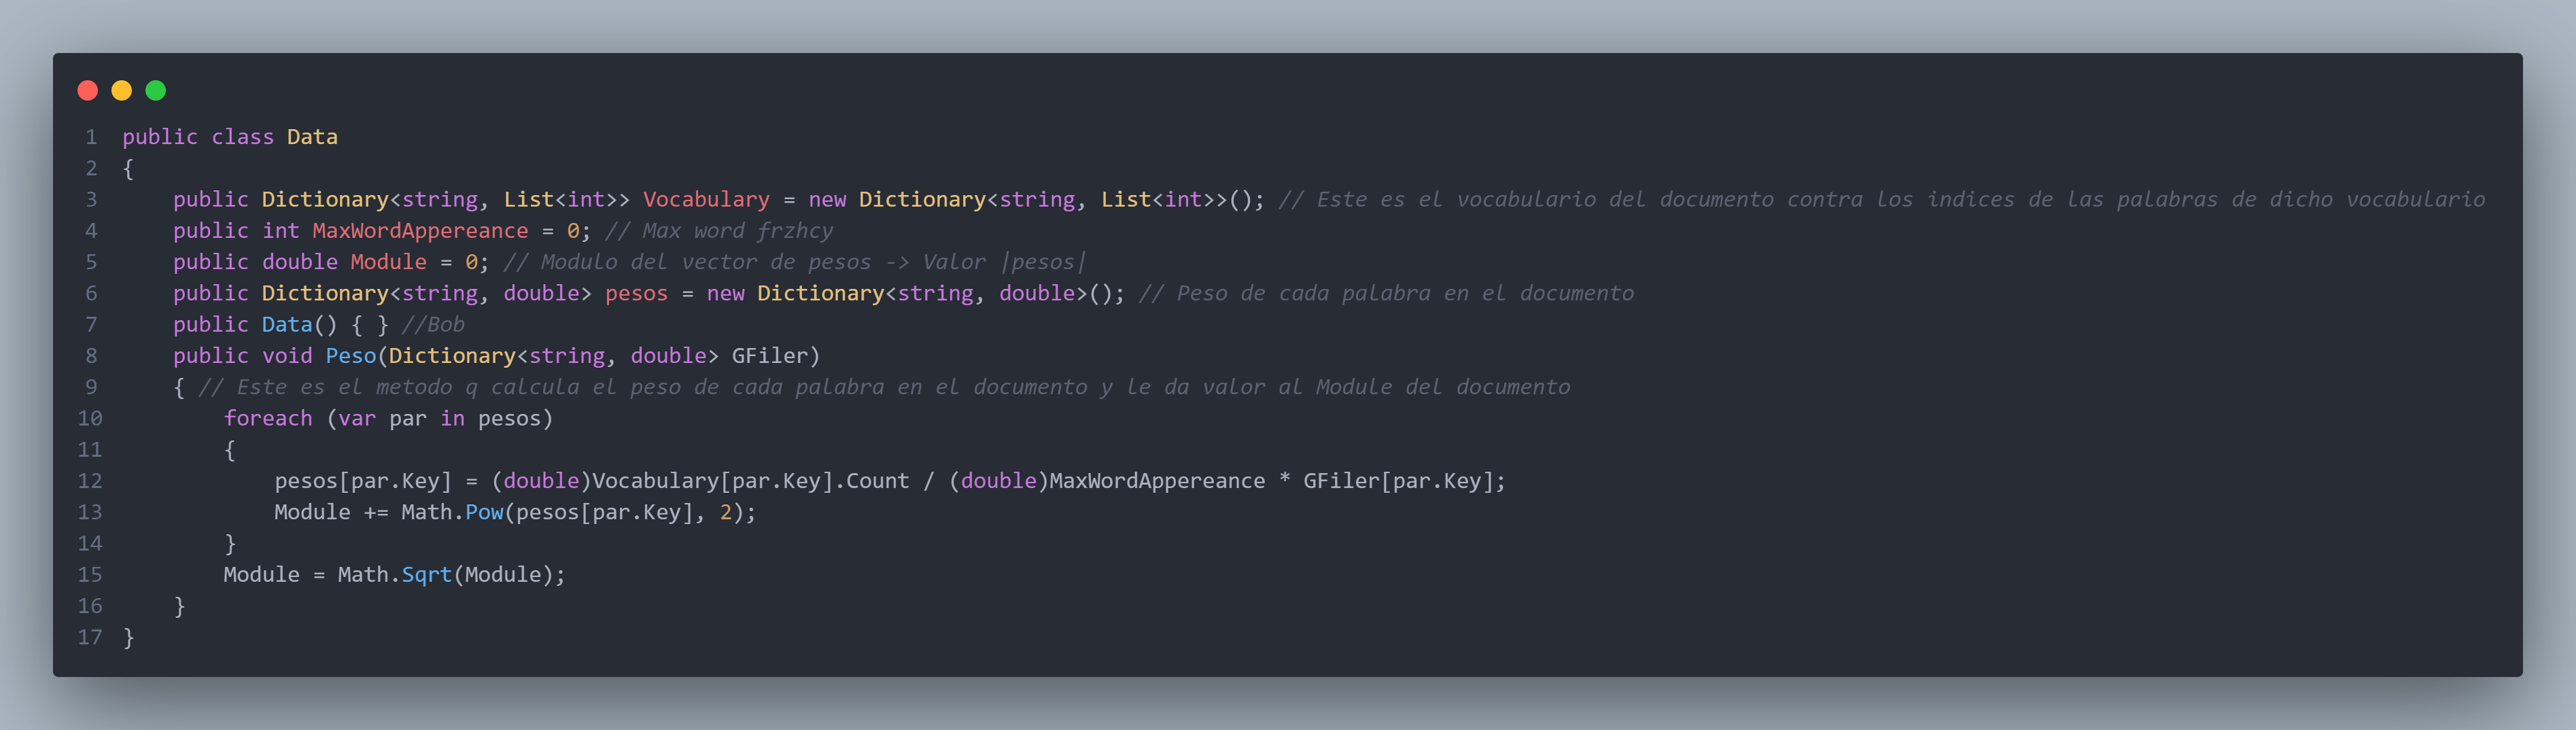
\includegraphics[width=310px, height=120px]{Assets/data_filer.png}
    \end{figure}
    Esta clase es la encargada de ir almacenando, como su nombre indica, los datos de cada documentos, que datos son estos?
    Pues son las palabras presentes de, cada documento, además del peso de estas, que luego se usarían en la consulta.
\end{frame}

